% Options for packages loaded elsewhere
\PassOptionsToPackage{unicode}{hyperref}
\PassOptionsToPackage{hyphens}{url}
%
\documentclass[
]{article}
\usepackage{amsmath,amssymb}
\usepackage{iftex}
\ifPDFTeX
  \usepackage[T1]{fontenc}
  \usepackage[utf8]{inputenc}
  \usepackage{textcomp} % provide euro and other symbols
\else % if luatex or xetex
  \usepackage{unicode-math} % this also loads fontspec
  \defaultfontfeatures{Scale=MatchLowercase}
  \defaultfontfeatures[\rmfamily]{Ligatures=TeX,Scale=1}
\fi
\usepackage{lmodern}
\ifPDFTeX\else
  % xetex/luatex font selection
\fi
% Use upquote if available, for straight quotes in verbatim environments
\IfFileExists{upquote.sty}{\usepackage{upquote}}{}
\IfFileExists{microtype.sty}{% use microtype if available
  \usepackage[]{microtype}
  \UseMicrotypeSet[protrusion]{basicmath} % disable protrusion for tt fonts
}{}
\makeatletter
\@ifundefined{KOMAClassName}{% if non-KOMA class
  \IfFileExists{parskip.sty}{%
    \usepackage{parskip}
  }{% else
    \setlength{\parindent}{0pt}
    \setlength{\parskip}{6pt plus 2pt minus 1pt}}
}{% if KOMA class
  \KOMAoptions{parskip=half}}
\makeatother
\usepackage{xcolor}
\usepackage[margin=1in]{geometry}
\usepackage{color}
\usepackage{fancyvrb}
\newcommand{\VerbBar}{|}
\newcommand{\VERB}{\Verb[commandchars=\\\{\}]}
\DefineVerbatimEnvironment{Highlighting}{Verbatim}{commandchars=\\\{\}}
% Add ',fontsize=\small' for more characters per line
\usepackage{framed}
\definecolor{shadecolor}{RGB}{248,248,248}
\newenvironment{Shaded}{\begin{snugshade}}{\end{snugshade}}
\newcommand{\AlertTok}[1]{\textcolor[rgb]{0.94,0.16,0.16}{#1}}
\newcommand{\AnnotationTok}[1]{\textcolor[rgb]{0.56,0.35,0.01}{\textbf{\textit{#1}}}}
\newcommand{\AttributeTok}[1]{\textcolor[rgb]{0.13,0.29,0.53}{#1}}
\newcommand{\BaseNTok}[1]{\textcolor[rgb]{0.00,0.00,0.81}{#1}}
\newcommand{\BuiltInTok}[1]{#1}
\newcommand{\CharTok}[1]{\textcolor[rgb]{0.31,0.60,0.02}{#1}}
\newcommand{\CommentTok}[1]{\textcolor[rgb]{0.56,0.35,0.01}{\textit{#1}}}
\newcommand{\CommentVarTok}[1]{\textcolor[rgb]{0.56,0.35,0.01}{\textbf{\textit{#1}}}}
\newcommand{\ConstantTok}[1]{\textcolor[rgb]{0.56,0.35,0.01}{#1}}
\newcommand{\ControlFlowTok}[1]{\textcolor[rgb]{0.13,0.29,0.53}{\textbf{#1}}}
\newcommand{\DataTypeTok}[1]{\textcolor[rgb]{0.13,0.29,0.53}{#1}}
\newcommand{\DecValTok}[1]{\textcolor[rgb]{0.00,0.00,0.81}{#1}}
\newcommand{\DocumentationTok}[1]{\textcolor[rgb]{0.56,0.35,0.01}{\textbf{\textit{#1}}}}
\newcommand{\ErrorTok}[1]{\textcolor[rgb]{0.64,0.00,0.00}{\textbf{#1}}}
\newcommand{\ExtensionTok}[1]{#1}
\newcommand{\FloatTok}[1]{\textcolor[rgb]{0.00,0.00,0.81}{#1}}
\newcommand{\FunctionTok}[1]{\textcolor[rgb]{0.13,0.29,0.53}{\textbf{#1}}}
\newcommand{\ImportTok}[1]{#1}
\newcommand{\InformationTok}[1]{\textcolor[rgb]{0.56,0.35,0.01}{\textbf{\textit{#1}}}}
\newcommand{\KeywordTok}[1]{\textcolor[rgb]{0.13,0.29,0.53}{\textbf{#1}}}
\newcommand{\NormalTok}[1]{#1}
\newcommand{\OperatorTok}[1]{\textcolor[rgb]{0.81,0.36,0.00}{\textbf{#1}}}
\newcommand{\OtherTok}[1]{\textcolor[rgb]{0.56,0.35,0.01}{#1}}
\newcommand{\PreprocessorTok}[1]{\textcolor[rgb]{0.56,0.35,0.01}{\textit{#1}}}
\newcommand{\RegionMarkerTok}[1]{#1}
\newcommand{\SpecialCharTok}[1]{\textcolor[rgb]{0.81,0.36,0.00}{\textbf{#1}}}
\newcommand{\SpecialStringTok}[1]{\textcolor[rgb]{0.31,0.60,0.02}{#1}}
\newcommand{\StringTok}[1]{\textcolor[rgb]{0.31,0.60,0.02}{#1}}
\newcommand{\VariableTok}[1]{\textcolor[rgb]{0.00,0.00,0.00}{#1}}
\newcommand{\VerbatimStringTok}[1]{\textcolor[rgb]{0.31,0.60,0.02}{#1}}
\newcommand{\WarningTok}[1]{\textcolor[rgb]{0.56,0.35,0.01}{\textbf{\textit{#1}}}}
\usepackage{longtable,booktabs,array}
\usepackage{calc} % for calculating minipage widths
% Correct order of tables after \paragraph or \subparagraph
\usepackage{etoolbox}
\makeatletter
\patchcmd\longtable{\par}{\if@noskipsec\mbox{}\fi\par}{}{}
\makeatother
% Allow footnotes in longtable head/foot
\IfFileExists{footnotehyper.sty}{\usepackage{footnotehyper}}{\usepackage{footnote}}
\makesavenoteenv{longtable}
\usepackage{graphicx}
\makeatletter
\def\maxwidth{\ifdim\Gin@nat@width>\linewidth\linewidth\else\Gin@nat@width\fi}
\def\maxheight{\ifdim\Gin@nat@height>\textheight\textheight\else\Gin@nat@height\fi}
\makeatother
% Scale images if necessary, so that they will not overflow the page
% margins by default, and it is still possible to overwrite the defaults
% using explicit options in \includegraphics[width, height, ...]{}
\setkeys{Gin}{width=\maxwidth,height=\maxheight,keepaspectratio}
% Set default figure placement to htbp
\makeatletter
\def\fps@figure{htbp}
\makeatother
\setlength{\emergencystretch}{3em} % prevent overfull lines
\providecommand{\tightlist}{%
  \setlength{\itemsep}{0pt}\setlength{\parskip}{0pt}}
\setcounter{secnumdepth}{-\maxdimen} % remove section numbering
\ifLuaTeX
  \usepackage{selnolig}  % disable illegal ligatures
\fi
\IfFileExists{bookmark.sty}{\usepackage{bookmark}}{\usepackage{hyperref}}
\IfFileExists{xurl.sty}{\usepackage{xurl}}{} % add URL line breaks if available
\urlstyle{same}
\hypersetup{
  pdftitle={ Examining Trends in Pediatric Healthcare Utilization },
  pdfauthor={ Laura Robles-Torres },
  hidelinks,
  pdfcreator={LaTeX via pandoc}}

\title{\strut \\
Examining Trends in Pediatric Healthcare Utilization\\}
\usepackage{etoolbox}
\makeatletter
\providecommand{\subtitle}[1]{% add subtitle to \maketitle
  \apptocmd{\@title}{\par {\large #1 \par}}{}{}
}
\makeatother
\subtitle{\\
Data Analyst Candidate Assignment: CCHSR\\}
\author{\strut \\
Laura Robles-Torres\\}
\date{\strut \\
February 18, 2025\\}

\begin{document}
\maketitle

\hypertarget{part-1-trends-in-utilization-of-various-healthcare-services-among-children-between-2015-and-2023}{%
\subsubsection{Part 1: Trends in utilization of various healthcare
services among children between 2015 and
2023}\label{part-1-trends-in-utilization-of-various-healthcare-services-among-children-between-2015-and-2023}}

\emph{The code below includes initial library loading, data importing,
and reshaping for analysis.}

\begin{Shaded}
\begin{Highlighting}[]
\FunctionTok{library}\NormalTok{(tidyverse)}
\FunctionTok{library}\NormalTok{(tidyr)}
\FunctionTok{library}\NormalTok{(readxl)}
\FunctionTok{library}\NormalTok{(dbplyr)}
\FunctionTok{library}\NormalTok{(stringr)}
\FunctionTok{library}\NormalTok{(sf)       }\CommentTok{\# For spatial data}
\FunctionTok{library}\NormalTok{(ggplot2)  }\CommentTok{\# For plotting}
\FunctionTok{library}\NormalTok{(tigris) }
\end{Highlighting}
\end{Shaded}

Initial data import

\begin{Shaded}
\begin{Highlighting}[]
\NormalTok{utilization\_data }\OtherTok{=}
\NormalTok{    readxl}\SpecialCharTok{::}\FunctionTok{read\_excel}\NormalTok{(}\StringTok{"data.xlsx"}\NormalTok{, }\AttributeTok{sheet =} \StringTok{"Sheet1"}\NormalTok{)}

\FunctionTok{head}\NormalTok{(utilization\_data)}
\end{Highlighting}
\end{Shaded}

Cleaning and shaping data for analysis

\begin{Shaded}
\begin{Highlighting}[]
\NormalTok{payor\_data }\OtherTok{=}\NormalTok{ utilization\_data }\SpecialCharTok{|\textgreater{}}
  \FunctionTok{mutate}\NormalTok{(}
    \AttributeTok{payor =} \FunctionTok{ifelse}\NormalTok{(category }\SpecialCharTok{\%in\%} \FunctionTok{c}\NormalTok{(}\StringTok{"Medicaid"}\NormalTok{, }\StringTok{"Private Insurance"}\NormalTok{), category, }\ConstantTok{NA}\NormalTok{)}
\NormalTok{  ) }\SpecialCharTok{|\textgreater{}} 
  \FunctionTok{fill}\NormalTok{(payor, }\AttributeTok{.direction =} \StringTok{"down"}\NormalTok{) }\SpecialCharTok{|\textgreater{}} 
  \FunctionTok{filter}\NormalTok{(}\SpecialCharTok{!}\NormalTok{category }\SpecialCharTok{\%in\%} \FunctionTok{c}\NormalTok{(}\StringTok{"Medicaid"}\NormalTok{, }\StringTok{"Private Insurance"}\NormalTok{)) }\SpecialCharTok{|\textgreater{}} \CommentTok{\# Remove payor label rows that are empty }
  \FunctionTok{slice}\NormalTok{(}\DecValTok{1}\SpecialCharTok{:}\DecValTok{8}\NormalTok{)}

\CommentTok{\# Reshape data into long format}
\NormalTok{payor\_data }\SpecialCharTok{|\textgreater{}}
  \FunctionTok{pivot\_longer}\NormalTok{(}\AttributeTok{cols =} \StringTok{\textasciigrave{}}\AttributeTok{2015}\StringTok{\textasciigrave{}}\SpecialCharTok{:}\StringTok{\textasciigrave{}}\AttributeTok{2023}\StringTok{\textasciigrave{}}\NormalTok{, }\AttributeTok{names\_to =} \StringTok{"year"}\NormalTok{, }\AttributeTok{values\_to =} \StringTok{"utilization"}\NormalTok{) }\SpecialCharTok{|\textgreater{}}
  \FunctionTok{mutate}\NormalTok{(}\AttributeTok{year =} \FunctionTok{as.numeric}\NormalTok{(year)) }\SpecialCharTok{|\textgreater{}}
  \FunctionTok{select}\NormalTok{(year, payor, category, utilization) }\OtherTok{{-}\textgreater{}}\NormalTok{ payor\_data}
\end{Highlighting}
\end{Shaded}

\hypertarget{utilization-of-different-healthcare-services-between-2015-and-2023}{%
\subsubsection{Utilization of different healthcare services between 2015
and
2023}\label{utilization-of-different-healthcare-services-between-2015-and-2023}}

Data collected group healthcare services by both \textbf{type of
service} and \textbf{insurance payers}. Healthcare services are grouped
in four different categories, listed below.

\begin{itemize}
\tightlist
\item
  Primary Care Visits, well-child
\item
  Primary Care Visits, sick
\item
  Emergency Department Visits
\item
  Inpatient Days
\end{itemize}

The insurance payers included are \textbf{Medicaid} and \textbf{Private
insurance}.

Between 2015 and 2023, several trends can be observed in healthcare
utilization among races/ethnicities and different payers.

\hypertarget{by-insurance-payor}{%
\paragraph{By insurance payor}\label{by-insurance-payor}}

Before 2020, trends in ED visits, primary care sick visits, and
inpatient days do not appear significantly different between the two
payer groups. However, more primary care well-child visits were covered
by private insurance than by Medicaid until 2020. Across all 4 types of
services, there is an increase in Medicaid as the primary payer starting
in 2020 with visits covered by private insurance remaining at a similar
level.

\begin{Shaded}
\begin{Highlighting}[]
\CommentTok{\#Plot utilization of each service by payor}
\FunctionTok{ggplot}\NormalTok{(payor\_data, }\FunctionTok{aes}\NormalTok{(}\AttributeTok{x =}\NormalTok{ year, }\AttributeTok{y =}\NormalTok{ utilization, }\AttributeTok{color =}\NormalTok{ payor)) }\SpecialCharTok{+}
  \FunctionTok{geom\_line}\NormalTok{() }\SpecialCharTok{+}
  \FunctionTok{facet\_wrap}\NormalTok{(}\SpecialCharTok{\textasciitilde{}}\NormalTok{ category, }\AttributeTok{scales =} \StringTok{"fixed"}\NormalTok{) }\SpecialCharTok{+}
  \FunctionTok{theme\_minimal}\NormalTok{() }\SpecialCharTok{+}
  \FunctionTok{labs}\NormalTok{(}\AttributeTok{title =} \StringTok{"Healthcare Utilization Trends by Payor"}\NormalTok{, }\AttributeTok{x =} \StringTok{"Year"}\NormalTok{, }\AttributeTok{y =} \StringTok{"Utilization"}\NormalTok{, }\AttributeTok{color=}\StringTok{"Insurance Payer"}\NormalTok{)}
\end{Highlighting}
\end{Shaded}

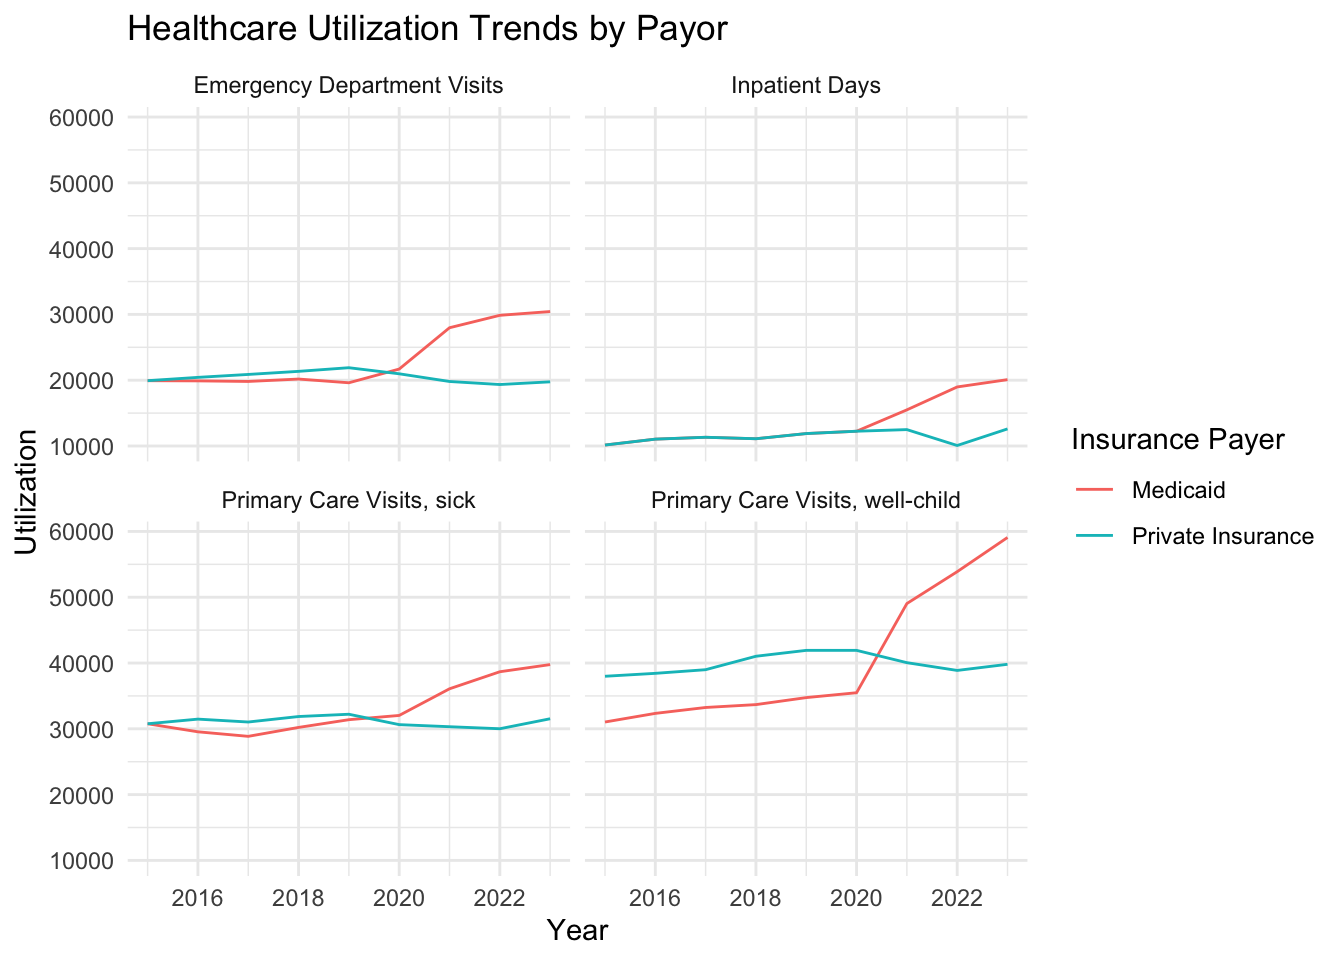
\includegraphics{mt-sinai-project_files/figure-latex/plotting payor trends-1.pdf}

This could be a reflection of Medicaid expansion initiatives that took
place in the wake of the COVID-19 pandemic starting in 2020. With more
individuals qualifying for Medicaid, more individuals were able to
access these 4 different types of healthcare services.

\hypertarget{by-raceethnicity}{%
\paragraph{By race/ethnicity}\label{by-raceethnicity}}

\begin{Shaded}
\begin{Highlighting}[]
\CommentTok{\#Clean data for racial group exploration}
\NormalTok{race\_data }\OtherTok{=} 
\NormalTok{  utilization\_data }\SpecialCharTok{|\textgreater{}}
  \FunctionTok{mutate}\NormalTok{(}
    \AttributeTok{race =} \FunctionTok{ifelse}\NormalTok{(category }\SpecialCharTok{\%in\%} \FunctionTok{c}\NormalTok{(}\StringTok{"Hispanic"}\NormalTok{, }\StringTok{"Non{-}Hispanic Black"}\NormalTok{, }\StringTok{"Non{-}Hispanic White"}\NormalTok{), category, }\ConstantTok{NA}\NormalTok{)}
\NormalTok{  ) }\SpecialCharTok{|\textgreater{}} 
  \FunctionTok{fill}\NormalTok{(race, }\AttributeTok{.direction =} \StringTok{"down"}\NormalTok{) }\SpecialCharTok{|\textgreater{}}  \CommentTok{\# Fill race downwards}
  \FunctionTok{filter}\NormalTok{(}\SpecialCharTok{!}\NormalTok{category }\SpecialCharTok{\%in\%} \FunctionTok{c}\NormalTok{(}\StringTok{"Hispanic"}\NormalTok{, }\StringTok{"Non{-}Hispanic Black"}\NormalTok{, }\StringTok{"Non{-}Hispanic White"}\NormalTok{)) }

\CommentTok{\# Reshape data into long format}
\NormalTok{race\_data }\SpecialCharTok{|\textgreater{}}
  \FunctionTok{pivot\_longer}\NormalTok{(}\AttributeTok{cols =} \StringTok{\textasciigrave{}}\AttributeTok{2015}\StringTok{\textasciigrave{}}\SpecialCharTok{:}\StringTok{\textasciigrave{}}\AttributeTok{2023}\StringTok{\textasciigrave{}}\NormalTok{, }\AttributeTok{names\_to =} \StringTok{"year"}\NormalTok{, }\AttributeTok{values\_to =} \StringTok{"utilization"}\NormalTok{)}\SpecialCharTok{|\textgreater{}}
  \FunctionTok{mutate}\NormalTok{(}\AttributeTok{year =} \FunctionTok{as.numeric}\NormalTok{(year)) }\SpecialCharTok{|\textgreater{}}
  \FunctionTok{filter}\NormalTok{(}\SpecialCharTok{!}\FunctionTok{is.na}\NormalTok{(utilization)) }\SpecialCharTok{|\textgreater{}}
  \FunctionTok{filter}\NormalTok{(}\SpecialCharTok{!}\FunctionTok{is.na}\NormalTok{(race)) }\SpecialCharTok{|\textgreater{}}
  \FunctionTok{slice\_tail}\NormalTok{(}\AttributeTok{n=}\DecValTok{126}\NormalTok{) }\OtherTok{{-}\textgreater{}}\NormalTok{ race\_data}
\end{Highlighting}
\end{Shaded}

For both ED visits and for inpatient days, Hispanic and Non-Hispanic
Black have a higher utilization than Non-Hispanic White children
overall. Since 2020, a slight decrease in ED visits for both of these
racial/ethnic groups can be observed. From 2015-2023, the number of
primary care well-child visits increased across all racial and ethnic
groups. However, Non-Hispanic White children still have a higher
utilization of this service than Hispanic and Non-Hispanic Black
children. Since 2020, the gap in primary care sick visits among the
different racial and ethnic groups seems to have decreased in comparison
with earlier years when Non-Hispnic Black and Hispanic children used
this service less than White children.

\begin{Shaded}
\begin{Highlighting}[]
\CommentTok{\#Plot utilization of each service by race/ethnicity}
\FunctionTok{ggplot}\NormalTok{(race\_data, }\FunctionTok{aes}\NormalTok{(}\AttributeTok{x =}\NormalTok{ year, }\AttributeTok{y =}\NormalTok{ utilization, }\AttributeTok{color =}\NormalTok{ race)) }\SpecialCharTok{+}
  \FunctionTok{geom\_line}\NormalTok{() }\SpecialCharTok{+}
  \FunctionTok{facet\_wrap}\NormalTok{(}\SpecialCharTok{\textasciitilde{}}\NormalTok{ category, }\AttributeTok{scales =} \StringTok{"fixed"}\NormalTok{) }\SpecialCharTok{+}
  \FunctionTok{theme\_minimal}\NormalTok{() }\SpecialCharTok{+}
  \FunctionTok{labs}\NormalTok{(}\AttributeTok{title =} \StringTok{"Healthcare Utilization Trends by Race/Ethnicity"}\NormalTok{, }\AttributeTok{x =} \StringTok{"Year"}\NormalTok{, }\AttributeTok{y =} \StringTok{"Utilization"}\NormalTok{, }\AttributeTok{color =} \StringTok{"Race/Ethnicity"}\NormalTok{)}
\end{Highlighting}
\end{Shaded}

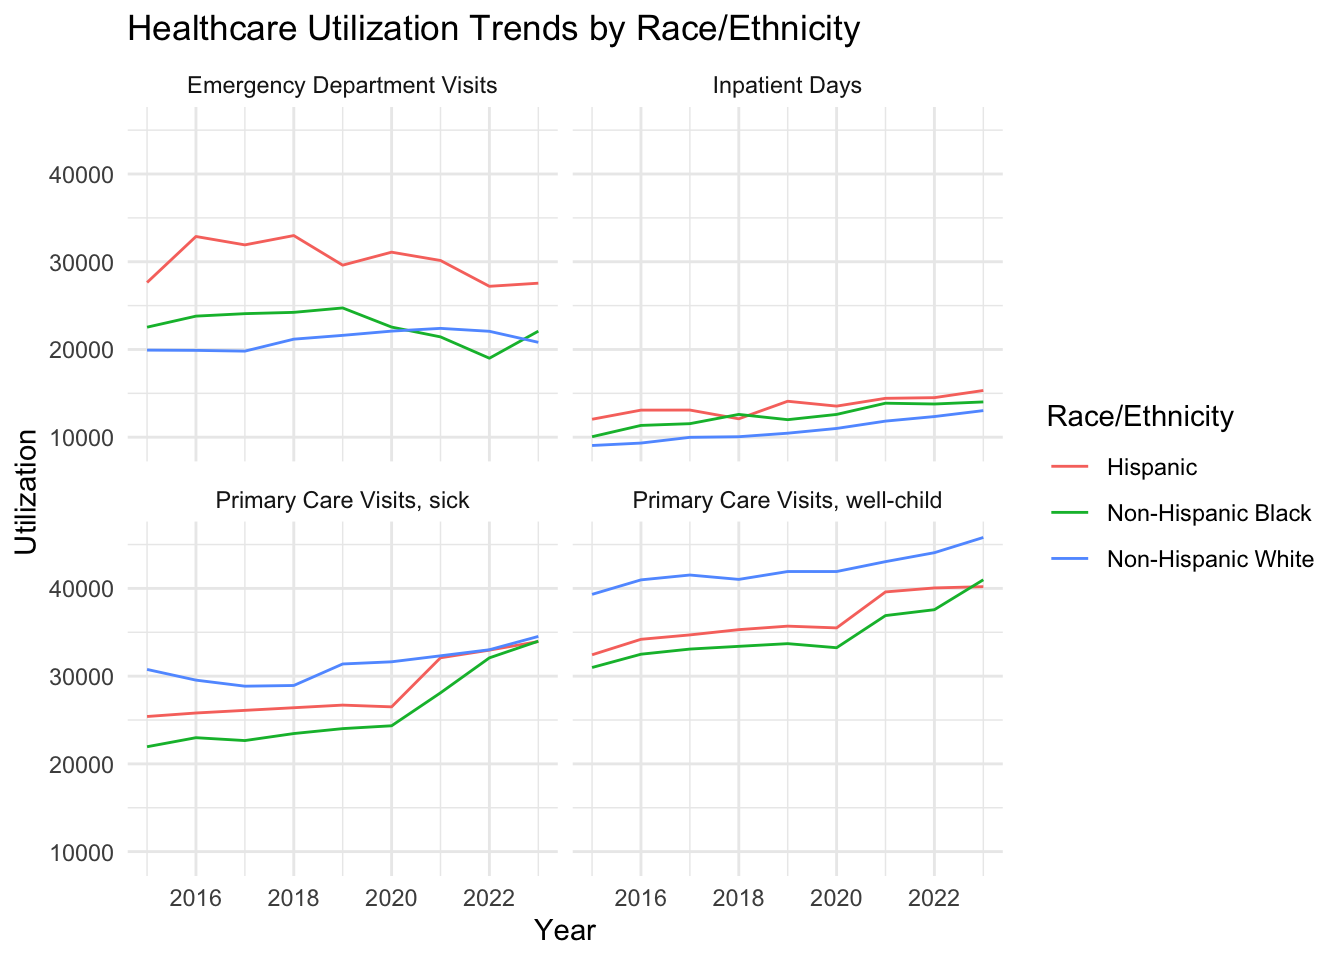
\includegraphics{mt-sinai-project_files/figure-latex/plotting racial trends-1.pdf}

\hypertarget{how-may-changes-to-medicaid-eligibility-requirements-impact-the-services-utilized-is-there-evidence-that-these-changes-differ-across-demographic-groups-hypothesize-potential-reasons-for-these-differences-if-so.}{%
\paragraph{How may changes to Medicaid eligibility requirements impact
the services utilized? Is there evidence that these changes differ
across demographic groups? Hypothesize potential reasons for these
differences if
so.}\label{how-may-changes-to-medicaid-eligibility-requirements-impact-the-services-utilized-is-there-evidence-that-these-changes-differ-across-demographic-groups-hypothesize-potential-reasons-for-these-differences-if-so.}}

Black and Hispanic children make up a majority of Medicaid enrolled
children in the United States. Since Medicaid is an income-based need
program, changes to Medicaid's eligibility system, particularly any
changes to the qualifying income level, may disproportionately impact
Black and Hispanic children. Decreasing the qualifying income level or
imposing work-requirements like some states have, for example, would
lead to less enrollees in Medicaid. If individuals that are enrolled
under expanded Medicaid eligibility have that eligibility rolled back,
it is likely that the trend observed since 2020 of increasing visits
covered by Medicaid would reverse.

The data show that Black and Hispanic children are less likely to go to
preventative well-child visits or primary care visits when sick, which
explains in part the higher ED utilization and higher inpatient days
observed by these groups, as they may have more severe illness by the
time they do seek care.

Overall, changes in Medicaid eligibility requirement would lead to a
decline in preventative \& routine care in a primary care environment
for Hispanic and Black children, that have historically had lower PC
utilization than White children, due to high out-of-pocket costs for
uninsured children. Such delay in seeking care when sick, for example,
will lead to an overrealiance on the ED and increase strains on
inpatient care.

\hypertarget{part-2-demographic-trends-among-children-who-underwent-surgery-for-congenital-heart-disease-in-ny-state-in-2022}{%
\subsubsection{Part 2: Demographic trends among children who underwent
surgery for congenital heart disease in NY state in
2022}\label{part-2-demographic-trends-among-children-who-underwent-surgery-for-congenital-heart-disease-in-ny-state-in-2022}}

\emph{The code below shows the importing and preparation of data for
linking.}

\begin{Shaded}
\begin{Highlighting}[]
\FunctionTok{options}\NormalTok{(}\AttributeTok{scipen =} \DecValTok{999}\NormalTok{)  }\CommentTok{\# Turn off scientific notation globally so data correctly imports from Excel sheet }

\NormalTok{sheet2 }\OtherTok{\textless{}{-}}\NormalTok{ readxl}\SpecialCharTok{::}\FunctionTok{read\_excel}\NormalTok{(}\StringTok{"data.xlsx"}\NormalTok{, }\AttributeTok{sheet =} \StringTok{"Sheet2"}\NormalTok{) }\CommentTok{\#Import sheet 2 (patient data)}

\NormalTok{sheet2}\SpecialCharTok{$}\NormalTok{tract }\OtherTok{\textless{}{-}} \FunctionTok{as.numeric}\NormalTok{(sheet2}\SpecialCharTok{$}\NormalTok{tract)  }\CommentTok{\# Convert \textquotesingle{}tract\textquotesingle{} column to numeric to facilitate join }

\CommentTok{\#import sheet 3}
\NormalTok{sheet3 }\OtherTok{\textless{}{-}}\NormalTok{ readxl}\SpecialCharTok{::}\FunctionTok{read\_excel}\NormalTok{(}\StringTok{"data.xlsx"}\NormalTok{, }\AttributeTok{sheet =} \StringTok{"Sheet3"}\NormalTok{) }\SpecialCharTok{|\textgreater{}}
\NormalTok{          janitor}\SpecialCharTok{::}\FunctionTok{clean\_names}\NormalTok{(}\AttributeTok{case =} \StringTok{"snake"}\NormalTok{) }\SpecialCharTok{|\textgreater{}} 
          \FunctionTok{separate}\NormalTok{(geo\_id, }\AttributeTok{sep=}\StringTok{"S"}\NormalTok{, }\AttributeTok{into =} \FunctionTok{c}\NormalTok{(}\StringTok{"geo\_id"}\NormalTok{, }\StringTok{"tract"}\NormalTok{)) }\SpecialCharTok{|\textgreater{}} \CommentTok{\#Extract \textquotesingle{}tract\textquotesingle{} from \textquotesingle{}geo\_id\textquotesingle{} variable for join }
          \FunctionTok{mutate}\NormalTok{(}\AttributeTok{tract =} \FunctionTok{as.numeric}\NormalTok{(tract)) }\CommentTok{\#Ensure tract is numeric as well }

\NormalTok{ clean\_sheet3 }\OtherTok{\textless{}{-}}\NormalTok{ sheet3 }\SpecialCharTok{|\textgreater{}} \CommentTok{\#Rename variables of interest for ease}
  \FunctionTok{rename}\NormalTok{(}\AttributeTok{pop\_6\_m=}\NormalTok{b27003\_003e, }\AttributeTok{pop\_18\_m =}\NormalTok{ b27003\_006e, }\AttributeTok{pop\_6\_f =}\NormalTok{ b27003\_031e, }\AttributeTok{pop\_18\_f =}\NormalTok{ b27003\_034e) }\SpecialCharTok{|\textgreater{}}
  \FunctionTok{rename}\NormalTok{(}\AttributeTok{public\_6\_m =}\NormalTok{ b27003\_004e, }\AttributeTok{public\_18\_m =}\NormalTok{ b27003\_007e, }\AttributeTok{public\_6\_f =}\NormalTok{ b27003\_032e, }\AttributeTok{public\_18\_f =}\NormalTok{ b27003\_035e) }\SpecialCharTok{|\textgreater{}} 
  \FunctionTok{select}\NormalTok{(}\SpecialCharTok{{-}}\NormalTok{geo\_id)}
 
\NormalTok{ clean\_sheet3 }\OtherTok{\textless{}{-}}\NormalTok{clean\_sheet3 }\SpecialCharTok{|\textgreater{}} \CommentTok{\#Select only variables of interest }
    \FunctionTok{select}\NormalTok{(tract, pop\_6\_m, pop\_18\_m,  pop\_6\_f, pop\_18\_f, public\_6\_m, }
\NormalTok{         public\_18\_m, public\_6\_f, public\_18\_f) }
\end{Highlighting}
\end{Shaded}

\emph{The code below shows the linking of data in Sheets 2 and 3.}

\begin{Shaded}
\begin{Highlighting}[]
\NormalTok{linked\_data }\OtherTok{=} 
  \FunctionTok{inner\_join}\NormalTok{(sheet2,clean\_sheet3, }\AttributeTok{by=}\FunctionTok{c}\NormalTok{(}\StringTok{"tract"}\NormalTok{))}
\end{Highlighting}
\end{Shaded}

\hypertarget{proportion-of-people-18-years-old-who-are-on-public-insurance-for-each-patients-census-tract}{%
\paragraph{Proportion of people ≤18 years old who are on public
insurance for each patient's census
tract:}\label{proportion-of-people-18-years-old-who-are-on-public-insurance-for-each-patients-census-tract}}

\emph{The table below is a sample to show final calculations.}

\begin{Shaded}
\begin{Highlighting}[]
\NormalTok{linked\_data }\SpecialCharTok{|\textgreater{}}
  \FunctionTok{mutate}\NormalTok{(}\AttributeTok{total\_pop =}\NormalTok{ pop\_6\_m }\SpecialCharTok{+}\NormalTok{ pop\_18\_m }\SpecialCharTok{+}\NormalTok{ pop\_6\_f }\SpecialCharTok{+}\NormalTok{ pop\_18\_f) }\SpecialCharTok{|\textgreater{}}
  \FunctionTok{mutate}\NormalTok{(}\AttributeTok{public\_pop =}\NormalTok{ public\_6\_m }\SpecialCharTok{+}\NormalTok{ public\_18\_m }\SpecialCharTok{+}\NormalTok{ public\_6\_f }\SpecialCharTok{+}\NormalTok{ public\_18\_f) }\SpecialCharTok{|\textgreater{}}
  \FunctionTok{mutate}\NormalTok{(}\AttributeTok{proportion\_public =}\NormalTok{ public\_pop }\SpecialCharTok{/}\NormalTok{ total\_pop) }\OtherTok{{-}\textgreater{}}\NormalTok{ proportion\_public\_per\_tract}

\NormalTok{sample\_proportion\_public }\OtherTok{\textless{}{-}}\NormalTok{ proportion\_public\_per\_tract }\SpecialCharTok{|\textgreater{}}
  \FunctionTok{distinct}\NormalTok{(tract, }\AttributeTok{.keep\_all =} \ConstantTok{TRUE}\NormalTok{) }\SpecialCharTok{|\textgreater{}}
  \FunctionTok{slice}\NormalTok{(}\DecValTok{1}\SpecialCharTok{:}\DecValTok{10}\NormalTok{) }\SpecialCharTok{|\textgreater{}} 
  \FunctionTok{select}\NormalTok{(patid, sex, age,race,tract,total\_pop,public\_pop, proportion\_public)}

\NormalTok{knitr}\SpecialCharTok{::}\FunctionTok{kable}\NormalTok{(sample\_proportion\_public)}
\end{Highlighting}
\end{Shaded}

\begin{longtable}[]{@{}
  >{\raggedleft\arraybackslash}p{(\columnwidth - 14\tabcolsep) * \real{0.0714}}
  >{\raggedleft\arraybackslash}p{(\columnwidth - 14\tabcolsep) * \real{0.0476}}
  >{\raggedleft\arraybackslash}p{(\columnwidth - 14\tabcolsep) * \real{0.0476}}
  >{\raggedright\arraybackslash}p{(\columnwidth - 14\tabcolsep) * \real{0.2262}}
  >{\raggedleft\arraybackslash}p{(\columnwidth - 14\tabcolsep) * \real{0.1429}}
  >{\raggedleft\arraybackslash}p{(\columnwidth - 14\tabcolsep) * \real{0.1190}}
  >{\raggedleft\arraybackslash}p{(\columnwidth - 14\tabcolsep) * \real{0.1310}}
  >{\raggedleft\arraybackslash}p{(\columnwidth - 14\tabcolsep) * \real{0.2143}}@{}}
\toprule\noalign{}
\begin{minipage}[b]{\linewidth}\raggedleft
patid
\end{minipage} & \begin{minipage}[b]{\linewidth}\raggedleft
sex
\end{minipage} & \begin{minipage}[b]{\linewidth}\raggedleft
age
\end{minipage} & \begin{minipage}[b]{\linewidth}\raggedright
race
\end{minipage} & \begin{minipage}[b]{\linewidth}\raggedleft
tract
\end{minipage} & \begin{minipage}[b]{\linewidth}\raggedleft
total\_pop
\end{minipage} & \begin{minipage}[b]{\linewidth}\raggedleft
public\_pop
\end{minipage} & \begin{minipage}[b]{\linewidth}\raggedleft
proportion\_public
\end{minipage} \\
\midrule\noalign{}
\endhead
\bottomrule\noalign{}
\endlastfoot
1 & 1 & 1 & Black non-Hispanic & 36001000100 & 740 & 600 & 0.8108108 \\
5 & 2 & 12 & Black non-Hispanic & 36001000201 & 463 & 390 & 0.8423326 \\
9 & 2 & 14 & Black non-Hispanic & 36001000202 & 659 & 526 & 0.7981791 \\
13 & 2 & 8 & Black non-Hispanic & 36001000301 & 738 & 444 & 0.6016260 \\
17 & 2 & 15 & Black non-Hispanic & 36001000302 & 511 & 286 &
0.5596869 \\
21 & 1 & 10 & Hispanic & 36001000401 & 141 & 10 & 0.0709220 \\
25 & 1 & 1 & Black non-Hispanic & 36001000403 & 467 & 226 & 0.4839400 \\
29 & 1 & 6 & Hispanic & 36001000404 & 1379 & 263 & 0.1907179 \\
33 & 1 & 14 & Black non-Hispanic & 36001000501 & 680 & 601 &
0.8838235 \\
37 & 1 & 14 & Black non-Hispanic & 36001000502 & 719 & 118 &
0.1641168 \\
\end{longtable}

\begin{Shaded}
\begin{Highlighting}[]
\FunctionTok{sum}\NormalTok{(}\FunctionTok{is.na}\NormalTok{(clean\_sheet3))}
\NormalTok{clean\_sheet3[}\SpecialCharTok{!}\FunctionTok{complete.cases}\NormalTok{(clean\_sheet3), ]}
\end{Highlighting}
\end{Shaded}

\hypertarget{patterns-by-public-insurance-and-raceethnicity}{%
\paragraph{Patterns by public insurance and
race/ethnicity}\label{patterns-by-public-insurance-and-raceethnicity}}

\hypertarget{our-sample-grouped-by-raceethnicity}{%
\subparagraph{Our sample grouped by
race/ethnicity}\label{our-sample-grouped-by-raceethnicity}}

\begin{Shaded}
\begin{Highlighting}[]
\CommentTok{\#how many children of each racial/ethnic group are in our dataset?}
\NormalTok{linked\_data }\SpecialCharTok{|\textgreater{}}
  \FunctionTok{group\_by}\NormalTok{(race) }\SpecialCharTok{|\textgreater{}}
  \FunctionTok{summarize}\NormalTok{(}\AttributeTok{n\_obs=}\FunctionTok{n}\NormalTok{()) }\SpecialCharTok{|\textgreater{}}
    \FunctionTok{arrange}\NormalTok{(}\FunctionTok{desc}\NormalTok{(n\_obs)) }\OtherTok{{-}\textgreater{}}\NormalTok{ grouped\_race }\CommentTok{\#we have a pretty balanced sample}

\NormalTok{knitr}\SpecialCharTok{::}\FunctionTok{kable}\NormalTok{(grouped\_race)}
\end{Highlighting}
\end{Shaded}

\begin{longtable}[]{@{}lr@{}}
\toprule\noalign{}
race & n\_obs \\
\midrule\noalign{}
\endhead
\bottomrule\noalign{}
\endlastfoot
Black non-Hispanic & 3400 \\
White non-Hispanic & 3212 \\
Hispanic & 2904 \\
\end{longtable}

\hypertarget{do-certain-racialethnic-groups-tend-to-have-higher-proportions-of-public-insurance}{%
\subparagraph{Do certain racial/ethnic groups tend to have higher
proportions of public
insurance?}\label{do-certain-racialethnic-groups-tend-to-have-higher-proportions-of-public-insurance}}

These are the top 25 census tracts with the highest proportion of people
\textless18 years old on public insurance:

\begin{Shaded}
\begin{Highlighting}[]
\NormalTok{proportion\_public\_per\_tract }\SpecialCharTok{|\textgreater{}}
  \FunctionTok{group\_by}\NormalTok{(tract) }\SpecialCharTok{|\textgreater{}}
  \FunctionTok{arrange}\NormalTok{(}\FunctionTok{desc}\NormalTok{(proportion\_public))}
\end{Highlighting}
\end{Shaded}

\begin{Shaded}
\begin{Highlighting}[]
\NormalTok{proportion\_public\_table\_unique }\OtherTok{\textless{}{-}}\NormalTok{ proportion\_public\_per\_tract }\SpecialCharTok{|\textgreater{}} 
  \FunctionTok{distinct}\NormalTok{(tract, }\AttributeTok{.keep\_all =} \ConstantTok{TRUE}\NormalTok{) }\SpecialCharTok{|\textgreater{}}
  \FunctionTok{arrange}\NormalTok{(}\FunctionTok{desc}\NormalTok{(proportion\_public)) }\SpecialCharTok{|\textgreater{}}
  \FunctionTok{slice}\NormalTok{(}\DecValTok{1}\SpecialCharTok{:}\DecValTok{25}\NormalTok{) }\SpecialCharTok{|\textgreater{}}
  \FunctionTok{select}\NormalTok{(patid, race, tract,proportion\_public)}

\NormalTok{knitr}\SpecialCharTok{::}\FunctionTok{kable}\NormalTok{(proportion\_public\_table\_unique)}
\end{Highlighting}
\end{Shaded}

\begin{longtable}[]{@{}rlrr@{}}
\toprule\noalign{}
patid & race & tract & proportion\_public \\
\midrule\noalign{}
\endhead
\bottomrule\noalign{}
\endlastfoot
973 & Black non-Hispanic & 36005021301 & 1.0000000 \\
1005 & Black non-Hispanic & 36005021900 & 1.0000000 \\
1085 & Black non-Hispanic & 36005023302 & 1.0000000 \\
1241 & Black non-Hispanic & 36005027600 & 1.0000000 \\
3157 & Black non-Hispanic & 36027220102 & 1.0000000 \\
3197 & Hispanic & 36027610000 & 1.0000000 \\
3245 & Black non-Hispanic & 36029001403 & 1.0000000 \\
3281 & Black non-Hispanic & 36029002502 & 1.0000000 \\
3509 & Black non-Hispanic & 36029007102 & 1.0000000 \\
3905 & Black non-Hispanic & 36029016300 & 1.0000000 \\
4000 & Hispanic & 36029980300 & 1.0000000 \\
4218 & Black non-Hispanic & 36037940100 & 1.0000000 \\
4567 & Black non-Hispanic & 36047028501 & 1.0000000 \\
4729 & Black non-Hispanic & 36047045300 & 1.0000000 \\
6444 & Black non-Hispanic & 36061009400 & 1.0000000 \\
8592 & Black non-Hispanic & 36093021001 & 1.0000000 \\
9266 & Black non-Hispanic & 36119000404 & 1.0000000 \\
9277 & Black non-Hispanic & 36119001000 & 1.0000000 \\
9356 & Black non-Hispanic & 36119006302 & 1.0000000 \\
1881 & Black non-Hispanic & 36007001100 & 0.9974684 \\
793 & Black non-Hispanic & 36005015500 & 0.9961089 \\
4507 & Black non-Hispanic & 36047022200 & 0.9950739 \\
4403 & Black non-Hispanic & 36047010802 & 0.9885808 \\
4740 & Black non-Hispanic & 36047047400 & 0.9822064 \\
8456 & Black non-Hispanic & 36087012110 & 0.9820412 \\
\end{longtable}

\textbf{The mean proportion of public health insurance coverage is
highest for Non-Hispanic Black children (65\%), compared to Hispanic
(35\%) and White (27\%) children.}

\begin{Shaded}
\begin{Highlighting}[]
\CommentTok{\#compare the mean proportion of children on public health insurance by racial group }
\NormalTok{proportion\_public\_per\_tract}\SpecialCharTok{|\textgreater{}}
  \FunctionTok{group\_by}\NormalTok{(race) }\SpecialCharTok{|\textgreater{}}
  \FunctionTok{summarise}\NormalTok{(}
    \AttributeTok{mean\_public\_ins =} \FunctionTok{mean}\NormalTok{(proportion\_public, }\AttributeTok{na.rm =} \ConstantTok{TRUE}\NormalTok{),}
    \AttributeTok{median\_public\_ins =} \FunctionTok{median}\NormalTok{(proportion\_public, }\AttributeTok{na.rm =} \ConstantTok{TRUE}\NormalTok{),}
    \AttributeTok{sd\_public\_ins =} \FunctionTok{sd}\NormalTok{(proportion\_public, }\AttributeTok{na.rm =} \ConstantTok{TRUE}\NormalTok{),}
    \AttributeTok{count =} \FunctionTok{n}\NormalTok{()}
\NormalTok{  ) }\OtherTok{{-}\textgreater{}}\NormalTok{ descriptive\_statistics}

\NormalTok{knitr}\SpecialCharTok{::}\FunctionTok{kable}\NormalTok{(descriptive\_statistics)}
\end{Highlighting}
\end{Shaded}

\begin{longtable}[]{@{}
  >{\raggedright\arraybackslash}p{(\columnwidth - 8\tabcolsep) * \real{0.2603}}
  >{\raggedleft\arraybackslash}p{(\columnwidth - 8\tabcolsep) * \real{0.2192}}
  >{\raggedleft\arraybackslash}p{(\columnwidth - 8\tabcolsep) * \real{0.2466}}
  >{\raggedleft\arraybackslash}p{(\columnwidth - 8\tabcolsep) * \real{0.1918}}
  >{\raggedleft\arraybackslash}p{(\columnwidth - 8\tabcolsep) * \real{0.0822}}@{}}
\toprule\noalign{}
\begin{minipage}[b]{\linewidth}\raggedright
race
\end{minipage} & \begin{minipage}[b]{\linewidth}\raggedleft
mean\_public\_ins
\end{minipage} & \begin{minipage}[b]{\linewidth}\raggedleft
median\_public\_ins
\end{minipage} & \begin{minipage}[b]{\linewidth}\raggedleft
sd\_public\_ins
\end{minipage} & \begin{minipage}[b]{\linewidth}\raggedleft
count
\end{minipage} \\
\midrule\noalign{}
\endhead
\bottomrule\noalign{}
\endlastfoot
Black non-Hispanic & 0.6278824 & 0.6547927 & 0.2182348 & 3400 \\
Hispanic & 0.3512884 & 0.3329493 & 0.2038245 & 2904 \\
White non-Hispanic & 0.2773984 & 0.2130841 & 0.2289701 & 3212 \\
\end{longtable}

\begin{Shaded}
\begin{Highlighting}[]
\FunctionTok{library}\NormalTok{(ggplot2)}

\FunctionTok{ggplot}\NormalTok{(proportion\_public\_per\_tract, }\FunctionTok{aes}\NormalTok{(}\AttributeTok{x =}\NormalTok{ race, }\AttributeTok{y =}\NormalTok{ proportion\_public, }\AttributeTok{fill =}\NormalTok{ race)) }\SpecialCharTok{+}
  \FunctionTok{geom\_boxplot}\NormalTok{() }\SpecialCharTok{+}
  \FunctionTok{labs}\NormalTok{(}\AttributeTok{title =} \StringTok{"Public Insurance Proportion by Race/Ethnicity"}\NormalTok{,}
       \AttributeTok{x =} \StringTok{"Race/Ethnicity"}\NormalTok{,}
       \AttributeTok{y =} \StringTok{"Proportion on Public Insurance"}\NormalTok{) }\SpecialCharTok{+}
  \FunctionTok{theme\_minimal}\NormalTok{() }\SpecialCharTok{+}
  \FunctionTok{theme}\NormalTok{(}\AttributeTok{axis.text.x =} \FunctionTok{element\_text}\NormalTok{(}\AttributeTok{angle =} \DecValTok{45}\NormalTok{, }\AttributeTok{hjust =} \DecValTok{1}\NormalTok{))}
\end{Highlighting}
\end{Shaded}

\includegraphics{mt-sinai-project_files/figure-latex/visualize-1.pdf}

\textbf{Black NH children are more likely to reside in census tracts
with a higher percentage of children on public insurance, while White NH
children are more likely to live in census tracts with lower public
insurance rates.}

A statistical test would be conducted to assess whether these
differences in public health insurance proportions between racial/ethnic
groups are statistically significant.

\end{document}
